\documentclass[11pt]{article}
%------------------------
%Packages
\usepackage[top=0.75in, bottom=1.25in, left=1in, right=1in]{geometry} 
\usepackage{amsmath,amsthm,amssymb} %this is THE math package
\usepackage{mathtools}
\usepackage{tikz}
\usepackage{graphicx}
\usepackage{enumitem}
\usepackage{fancybox}
\usepackage{hyperref}
\usepackage{varwidth}
\usepackage{mdframed}
\usepackage{mathrsfs}
%------------------------
%Fonts I use, uncomment if you like to use them.
%The first is the general font, and the second a math font
\usepackage{mathpazo}
%\usepackage{eulervm}
%------------------------
%This is so that we have standard fonts for the doublestroked symbols
%for reals, naturals etc. regardless of what font you use.
%Don't comment
\AtBeginDocument{
  \DeclareSymbolFont{AMSb}{U}{msb}{m}{n}
  \DeclareSymbolFontAlphabet{\mathbb}{AMSb}}

%----------------------------------------------
%User-defined environments
%Commented because we're not using them in this document
%The only uncommented ones are the Problem and Solution environment

% \newenvironment{theorem}[2][Theorem]{\begin{trivlist}
% \item[\hskip \labelsep {\bfseries #1}\hskip \labelsep {\bfseries #2.}]}{\end{trivlist}}
% \newenvironment{lemma}[2][Lemma]{\begin{trivlist}
% \item[\hskip \labelsep {\bfseries #1}\hskip \labelsep {\bfseries #2.}]}{\end{trivlist}}
% \newenvironment{exercise}[2][Exercise]{\begin{trivlist}
% \item[\hskip \labelsep {\bfseries #1}\hskip \labelsep {\bfseries #2.}]}{\end{trivlist}}
% \newenvironment{question}[2][Question]{\begin{trivlist}
% \item[\hskip \labelsep {\bfseries #1}\hskip \labelsep {\bfseries #2.}]}{\end{trivlist}}
% \newenvironment{corollary}[2][Corollary]{\begin{trivlist}
% \item[\hskip \labelsep {\bfseries #1}\hskip \labelsep {\bfseries #2.}]}{\end{trivlist}}
\newenvironment{problem}[2][Problem\!]{\begin{trivlist}
\item[\hskip \labelsep {\bfseries #1}\hskip \labelsep {\bfseries #2.}]}{\end{trivlist}}
%\newenvironment{sub-problem}[2][]{\begin{trivlist}
%\item[\hskip \labelsep {\bfseries #1}\hskip \labelsep {\bfseries #2}]}{\end{trivlist}}
\newenvironment{solution}{\begin{proof}[\textbf{\textit{Solution}}]}{\end{proof}}
%----------------------------------------------

%----------------------------
%User-defined notations
\newcommand{\zz}{\mathbb Z}   %blackboard bold Z
\newcommand{\qq}{\mathbb Q}   %blackboard bold Q
\newcommand{\ff}{\mathbb F}   %blackboard bold F
\newcommand{\rr}{\mathbb R}   %blackboard bold R
\newcommand{\nn}{\mathbb N}   %blackboard bold N
\newcommand{\cc}{\mathbb C}   %blackboard bold C
\newcommand{\af}{\mathbb A}   %blackboard bold A
\newcommand{\pp}{\mathbb P}   %blackboard bold P
\newcommand{\id}{\operatorname{id}} %for identity map
\newcommand{\im}{\operatorname{im}} %for image of a function
\newcommand{\dom}{\operatorname{dom}} %for domain of a function
\newcommand{\cat}[1]{\mathscr{#1}}   %calligraphic category
\newcommand{\abs}[1]{\left\lvert#1\right\rvert} %for absolute value
\newcommand{\norm}[1]{\left\lVert#1\right\rVert} %for norm
\newcommand{\modar}[1]{\text{ mod }{#1}} %for modular arithmetic
\newcommand{\set}[1]{\left\{#1\right\}} %for set
\newcommand{\setp}[2]{\left\{#1\ \middle|\ #2\right\}} %for set with a property
\newcommand{\card}[1]{\#\,{#1}} %for cardinality of a set

%Re-defined notations
\renewcommand{\epsilon}{\varepsilon}
\renewcommand{\phi}{\varphi}
\renewcommand{\emptyset}{\varnothing}
\renewcommand{\geq}{\geqslant}
\renewcommand{\leq}{\leqslant}
\renewcommand{\Re}{\operatorname{Re}}
\renewcommand{\gcd}{\operatorname{GCD}}
\renewcommand{\Im}{\operatorname{Im}}
%----------------------------

\allowdisplaybreaks
 
\begin{document}
 
\title{Problem Set 1}
\author{[Keene Ho]\\[0.5em]
MATH 100 | Introduction to Proof and Problem Solving | Summer 2023}
\date{} 
\maketitle

%Use \[...\] instead of $$...$$

\begin{problem}{1.1}
Let 
\[A = \set{\set{\emptyset},d,\set{a,c},b}\]
\begin{itemize}[itemsep=3em]
\item[(a)] What is $\abs{A}$?
%----------------------------------------
\begin{solution}\hfill %Do not delete
\(|A|\) is \(4\). The set \(\set{\emptyset}\) is an element of \(A\). The \(d\) is also an element of \(A\). The set \(\set{a,c}\) is also an element of \(A\). The \(b\) is also an element of \(A\).
\end{solution}
%----------------------------------------

\item[(b)] Which of the following are \emph{elements} of $A$: $a,\ b,\ c,\ \set{d},\ \set{a,c},\ \set{\set{a,c},b},\ \emptyset,\ \set{\emptyset},\ \set{\set{\emptyset}}$?
%----------------------------------------
\begin{solution}\hfill %Do not delete
The element \(a\) is not in set \(A\). The element \(b\) is in set \(A\). The element \(c\) is not in set \(A\). The set \(\set{d}\) is not in \(A\). The set \(\set{a,c}\) is in \(A\). The set \(\set{\set{a,c},b}\) is not in \(A\). The element \(\emptyset\) is not in \(A\). The set \(\set{\emptyset}\) is in \(A\). The set \(\set{\set{\emptyset}}\) is not in \(A\). So the only elements of \(A\) are \(b\), \(\set{a,c}\) and \(\set{\emptyset}\).
\end{solution}
%----------------------------------------

\item[(c)] Which of the following are \emph{subsets} of $A$: $a,\ b,\ c,\ \set{d},\ \set{a,c},\ \set{\set{a,c},b},\ \emptyset,\ \set{\emptyset},\ \set{\set{\emptyset}}$?
%----------------------------------------
\begin{solution}\hfill %Do not delete
\(\set{d}\) is a subset of \(A\). \(\set{\set{a,c},b}\) is a subset of \(A\). \(\emptyset\) is a subset of \(A\). \(\set{\set{\emptyset}}\) is also a subset of \(A\).
\end{solution}
%----------------------------------------

\item[(d)] Can $A$ be the power set of some set?
%----------------------------------------
\begin{solution}\hfill %Do not delete
No, since it doesn't contain all possible subsets of its original set. All the elements would be sets.
\end{solution}
%----------------------------------------

%\item[(e)] Write down a partition of $A$.
%----------------------------------------
%\begin{solution}\hfill %Do not delete
%Uncomment and WRITE YOUR SOLUTION HERE
%\end{solution}
%----------------------------------------

\end{itemize}
\end{problem}

\newpage %Do not delete

\begin{problem}{1.2}
Let $A$ be as above, and let $B = \set{\set{1},\set{\emptyset},b,c}$. What is
\begin{itemize}[itemsep=3em]
\item[(a)] $A \cap B$?
%----------------------------------------
\begin{solution}\hfill %Do not delete
\(\set{\emptyset}\) and \(b\) since thats what both sets have.
\end{solution}
%----------------------------------------

\item[(b)] $A\, \triangle\, B$?
%----------------------------------------
\begin{solution}\hfill %Do not delete
Elements present in \(A\) or \(B\) but not both. So that would be \(\set{a,c}\), \(\set{1}\), \(d\), and \(c\).
\end{solution}
%----------------------------------------

\item[(c)] $\set{\set{1}}^c$ in $A\, \triangle\, B$?
%----------------------------------------
\begin{solution}\hfill %Do not delete
The \(\set{\set{1}}^c\) are the elements not including \({{1}}\) so that would be \(\set{a,c}\), \(d\), and \(c\).
\end{solution}
%----------------------------------------

\item[(d)] $(A \times B) \setminus \setp{(x,y) \in A \times B}{x = \set{\emptyset} \text{ or } y = \set{\emptyset}}$?
%----------------------------------------
\begin{solution}\hfill %Do not delete
\(A \times B\) = \{(\{\emptyset\}, \{1\}), (\{\emptyset\}, \{\emptyset\}), (\{\emptyset\}, b), (\{\emptyset\}, c),
             \\(d, \{1\}), (d, \{\emptyset\}), (d, b), (d, c),
             \\(\{a, c\}, \{1\}), (\{a, c\}, \{\emptyset\}), (\{a, c\}, b), (\{a, c\}, c),
             \\(b, \{1\}), (b, \{\emptyset\}), (b, b), (b, c) \}

             Then removed all the ordered pairs where \(x = \set{\emptyset}\) or \(y = \set{\emptyset}\).
\[A \times B = \{(d, \{1\}), (d, b), (d, c), (\{a, c\}, \{1\}), (\{a, c\}, b), (\{a, c\}, c), (b, \{1\}), (b, b), (b, c) \}\]
\end{solution}
%----------------------------------------

\end{itemize}
\end{problem}

\newpage  %Do not delete

\begin{problem}{1.3}
Let $X$ and $Y$ be sets. Prove that $X\, \triangle\, Y = (X \cup Y) \setminus (X \cap Y)$ using a Venn diagram. 
\end{problem}
%----------------------------------------
\begin{solution}\hfill %Do not delete
%Uncomment and WRITE YOUR SOLUTION HERE
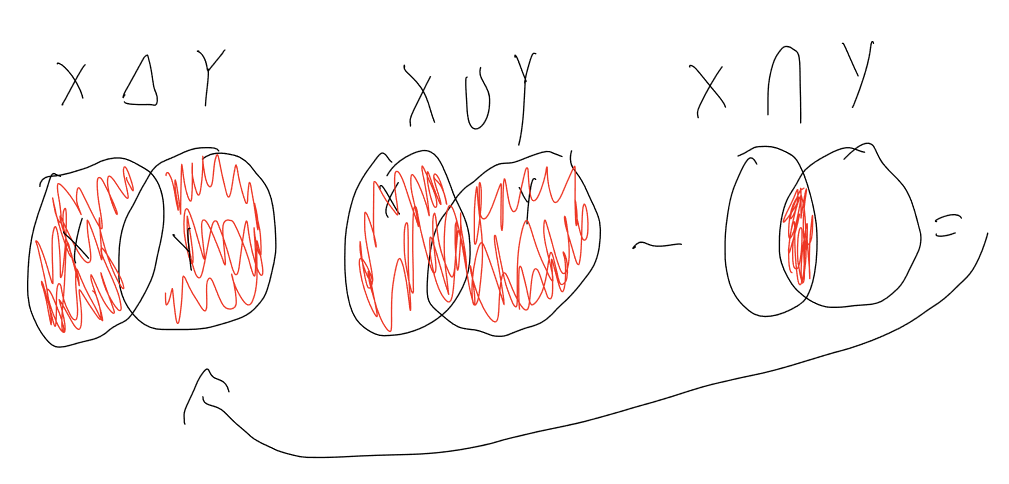
\includegraphics[scale=0.5]{Screenshot_14.png}
%to add graphics
\end{solution}
%----------------------------------------

\newpage  %Do not delete

\begin{center}
\textbf{Collaborators:}
%List your peers with whom you discussed the Problem Set
\end{center}
\vfill 

\begin{center}
\textbf{References:}
%List any book/website/notes that you used to write your solutions
\end{center}
\begin{itemize}
\item[$\bullet$] [Book(s): Title, Author]
\item[$\bullet$] [Online: \href{http://example.com/}{Link}]
\item[$\bullet$] [Notes: \href{http://example.com/}{Link}]
\end{itemize}

\vfill
%\begin{center}
%Fin.
%\end{center}
%\vfill

\end{document}